\chapter{Avaliação dos resultados do experimento}
	Ao executar o \textit{test bench} obteve-se os resultados conforme as
	\autoref{figura:testBenchWaveMaquina} e \autoref{figura:testBenchTranscriptMaquina}.

	\begin{figure}[H]
		 \centering
		 \caption{\label{figura:testBenchWaveMaquina}\textit{Test bench Wave} do código da máquina.}
		 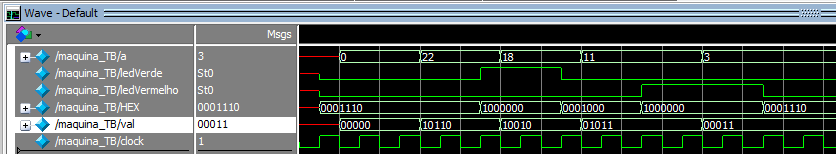
\includegraphics[width=1\textwidth]{img/maquina/testBenchWave}
	\end{figure}

	\begin{figure}[H]
		 \centering
		 \caption{\label{figura:testBenchTranscriptMaquina}\textit{Test bench Transcript} do código da máquina.}
		 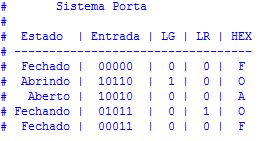
\includegraphics[width=0.5\textwidth]{img/maquina/testBenchTranscript}
	\end{figure}

	Como resultado do \textit{deploy} na placa, obteve o resultado confome a
	\autoref{figura:deployMaquina}

	\begin{figure}[H]
		\centering

		\begin{subfigure}[b]{0.44\textwidth}
			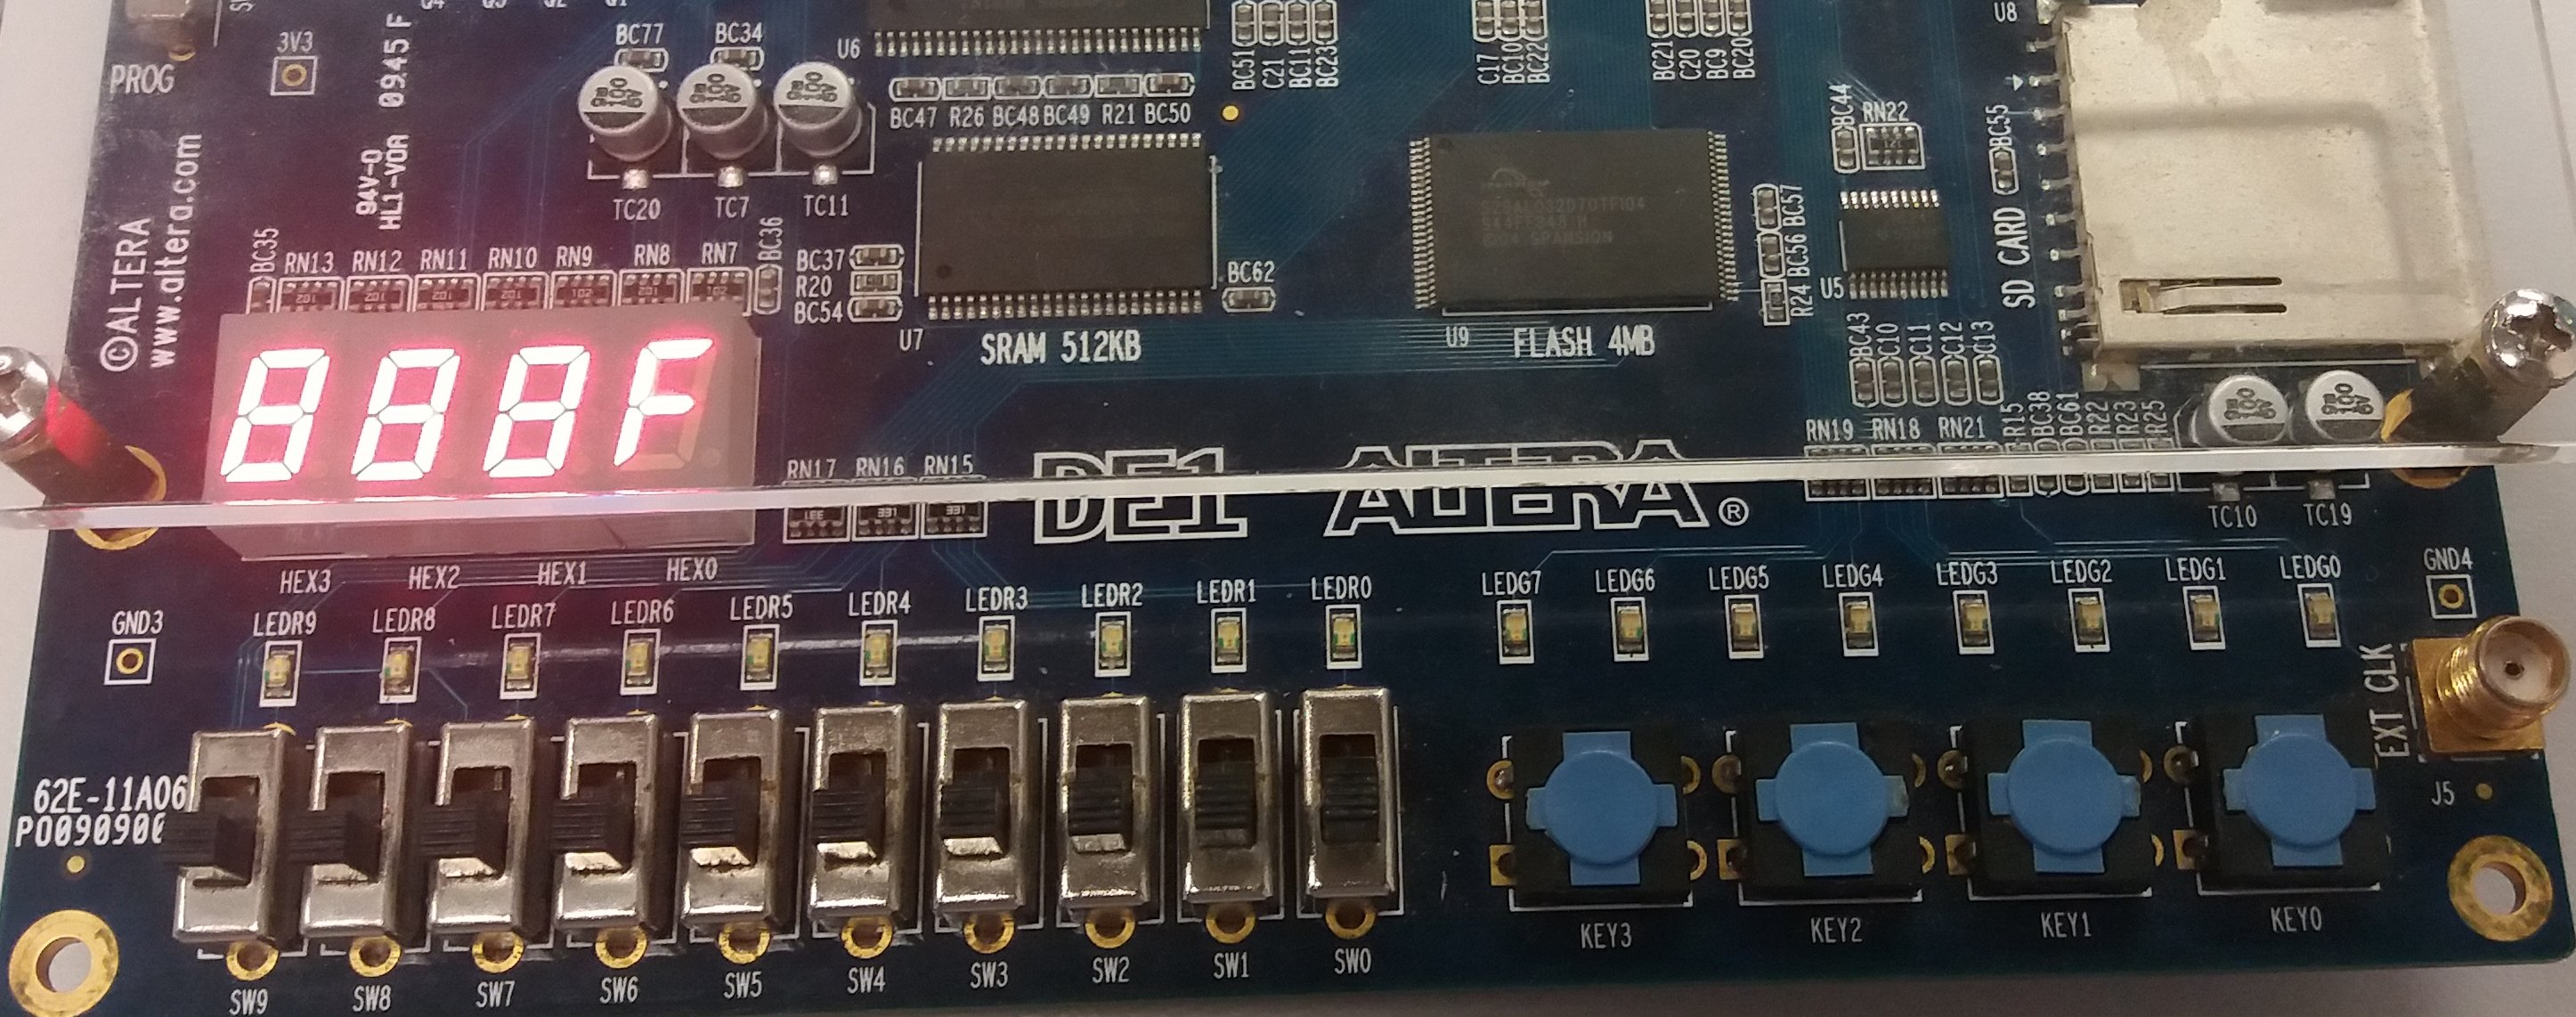
\includegraphics[width=\textwidth]{img/maquina/placa/Fechado}
			\caption{Máquina no estado inicial (Fechado).}
		\end{subfigure}
		~
		\begin{subfigure}[b]{0.44\textwidth}
			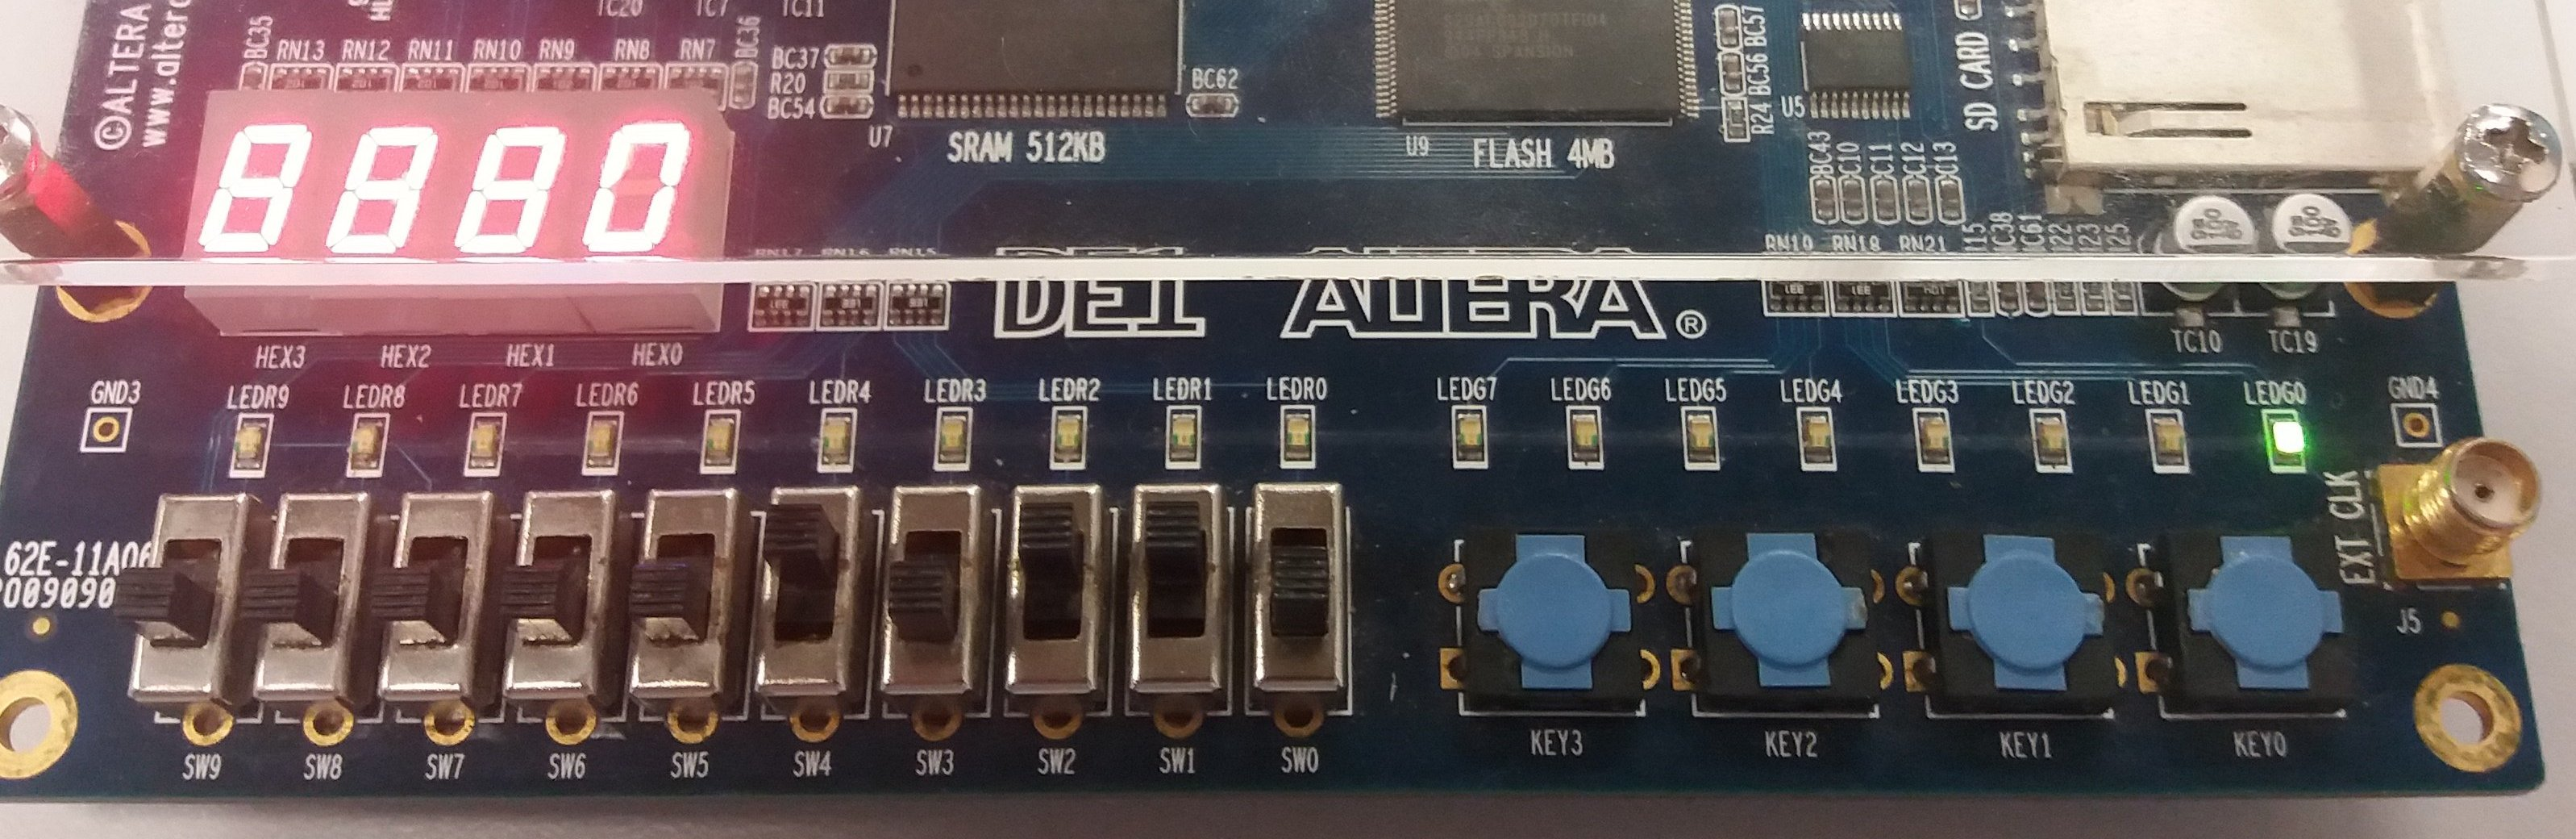
\includegraphics[width=\textwidth]{img/maquina/placa/Fechado-Abrindo}
			\caption{Transição do estado Fechado para o Abrindo.}
		\end{subfigure}

		\begin{subfigure}[b]{0.44\textwidth}
			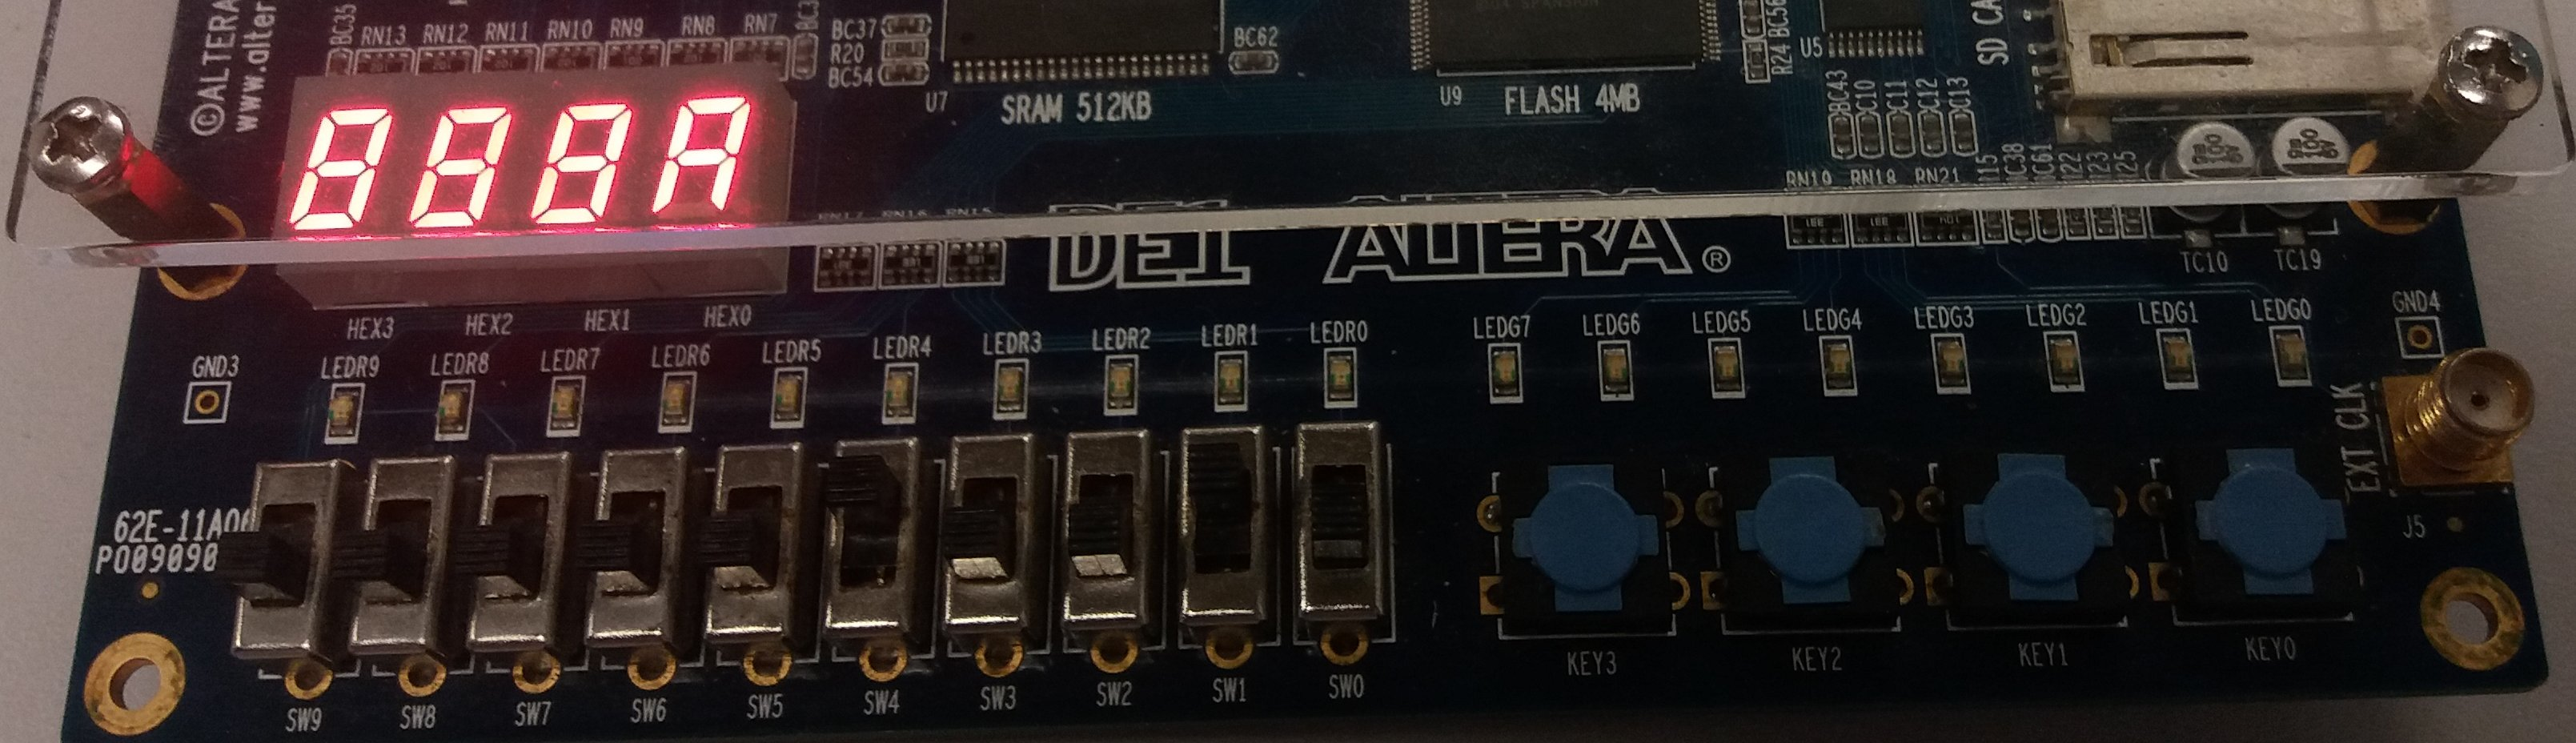
\includegraphics[width=\textwidth]{img/maquina/placa/Abrindo-Aberto}
			\caption{Transição do estado Abrindo para o Aberto.}
		\end{subfigure}
		~
		\begin{subfigure}[b]{0.44\textwidth}
			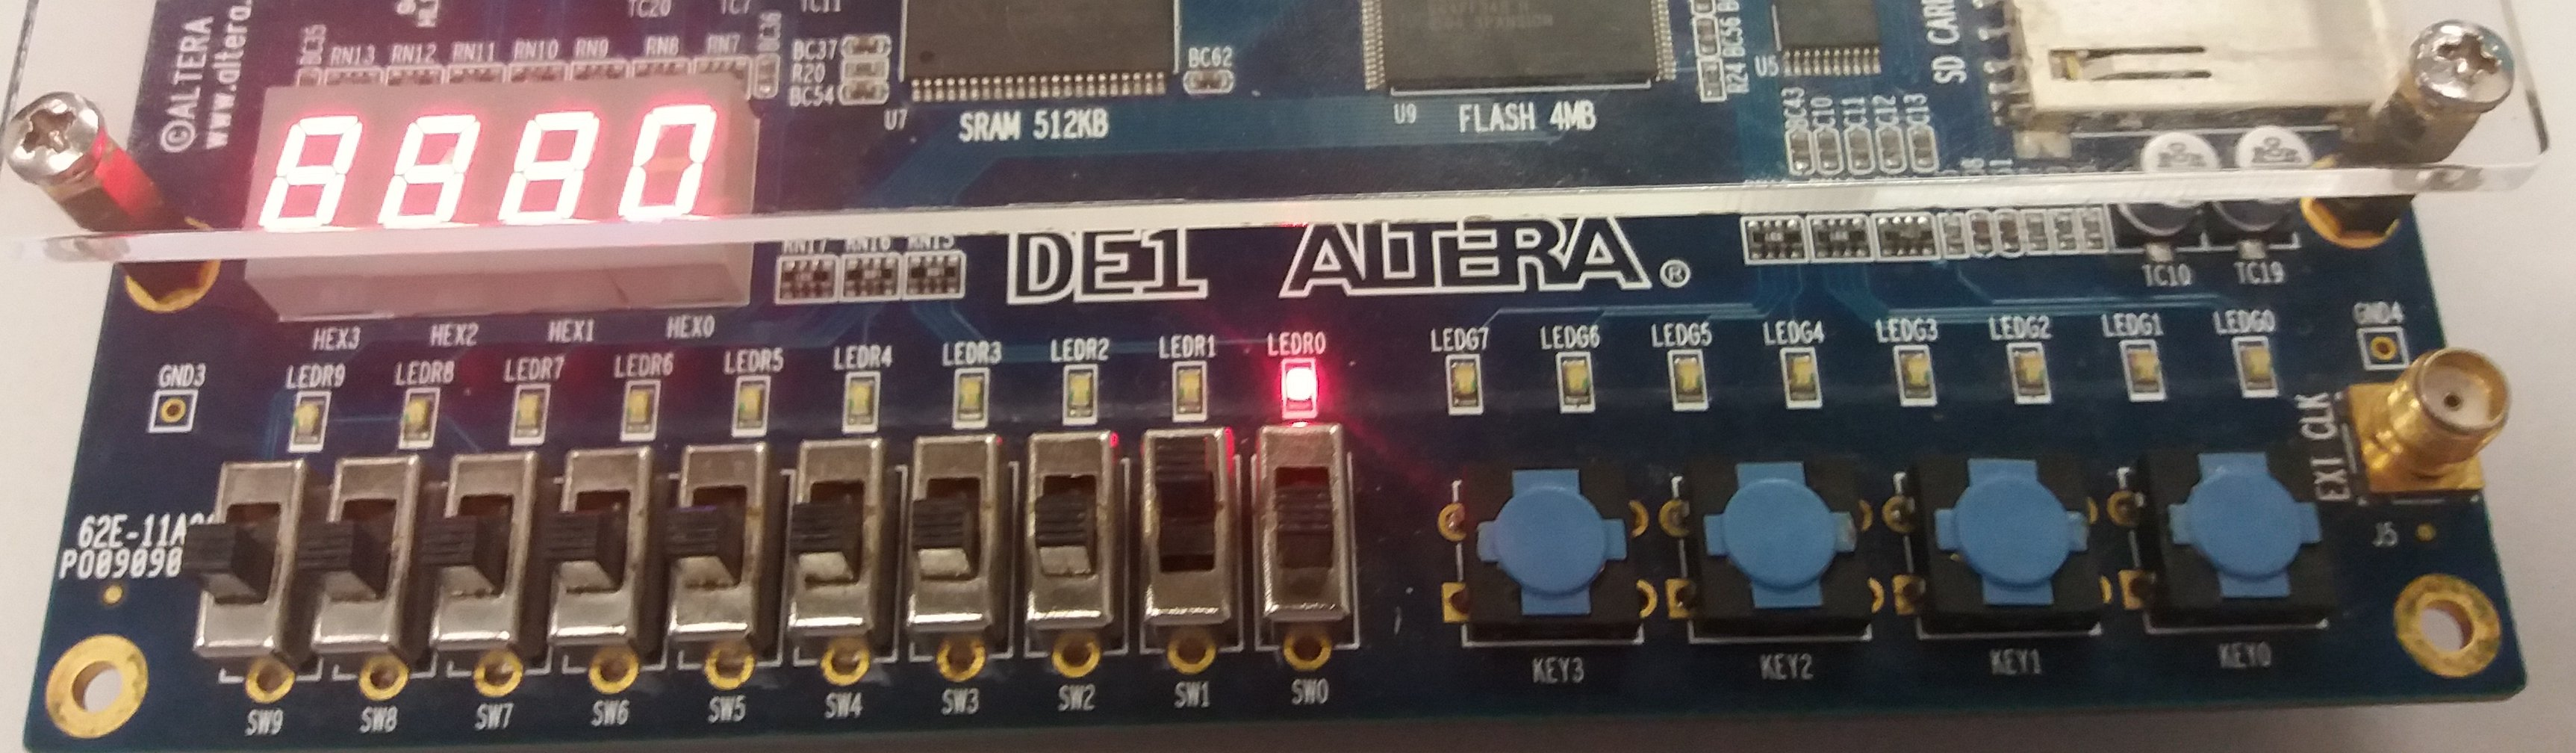
\includegraphics[width=\textwidth]{img/maquina/placa/Abrindo-Fechando}
			\caption{Transição do estado Abrindo para o Fechando.}
		\end{subfigure}

		\begin{subfigure}[b]{0.44\textwidth}
			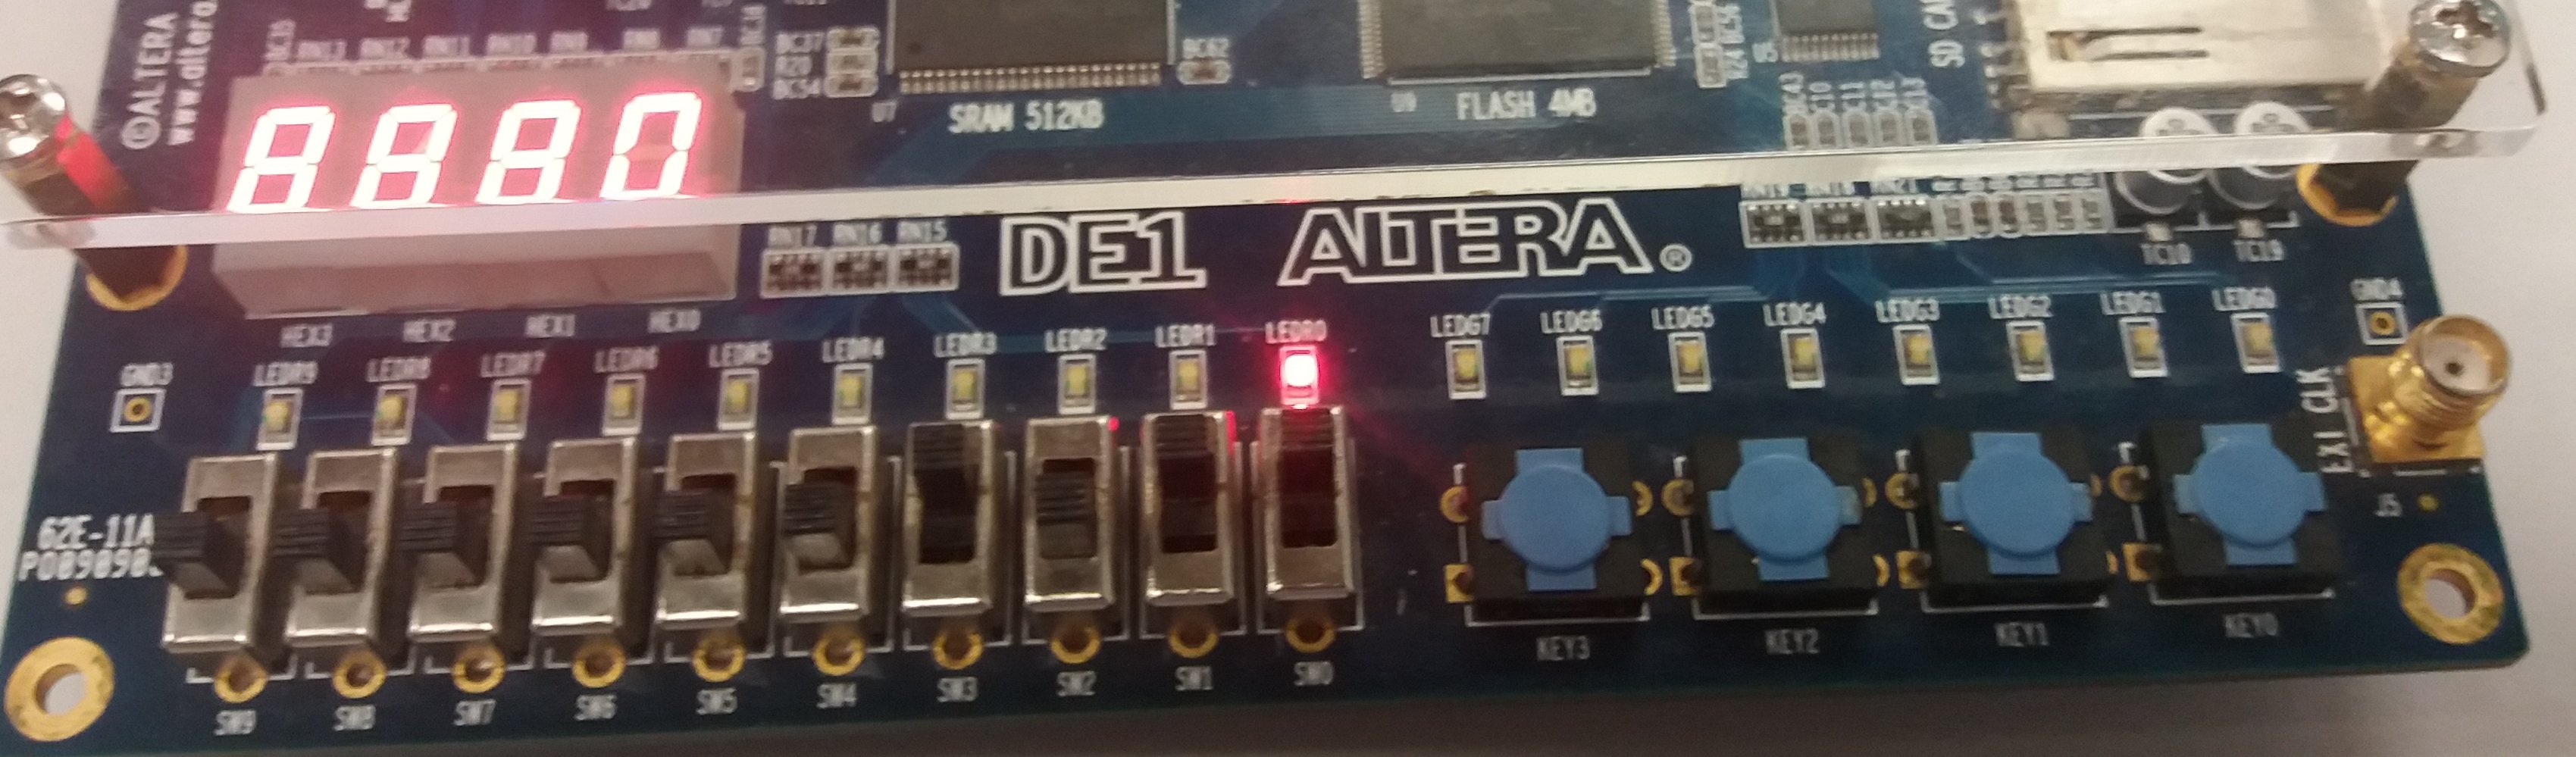
\includegraphics[width=\textwidth]{img/maquina/placa/Aberto-Fechando}
			\caption{Transição do estado Aberto para o Fechando.}
		\end{subfigure}
		~
		\begin{subfigure}[b]{0.44\textwidth}
			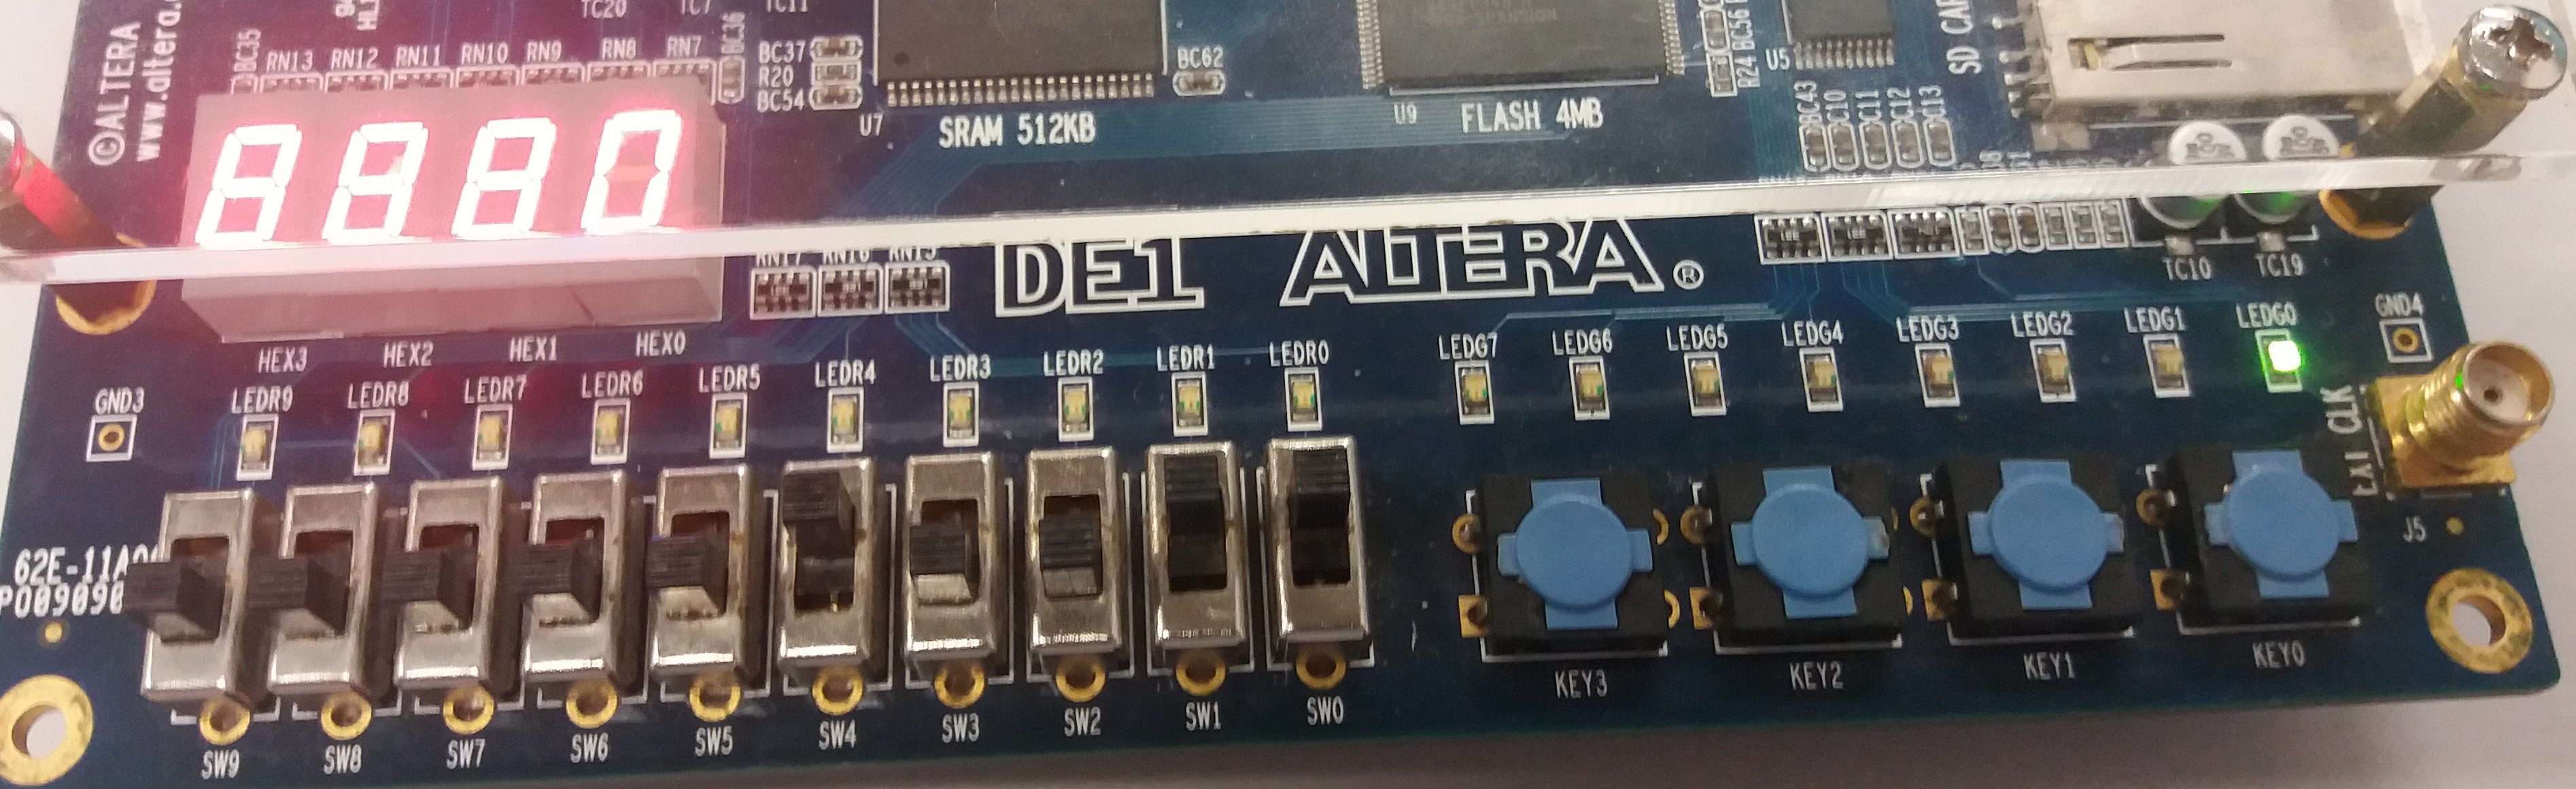
\includegraphics[width=\textwidth]{img/maquina/placa/Fechando-Abrindo}
			\caption{Transição do estado Fechando para Abrindo.}
		\end{subfigure}

		\begin{subfigure}[b]{0.44\textwidth}
			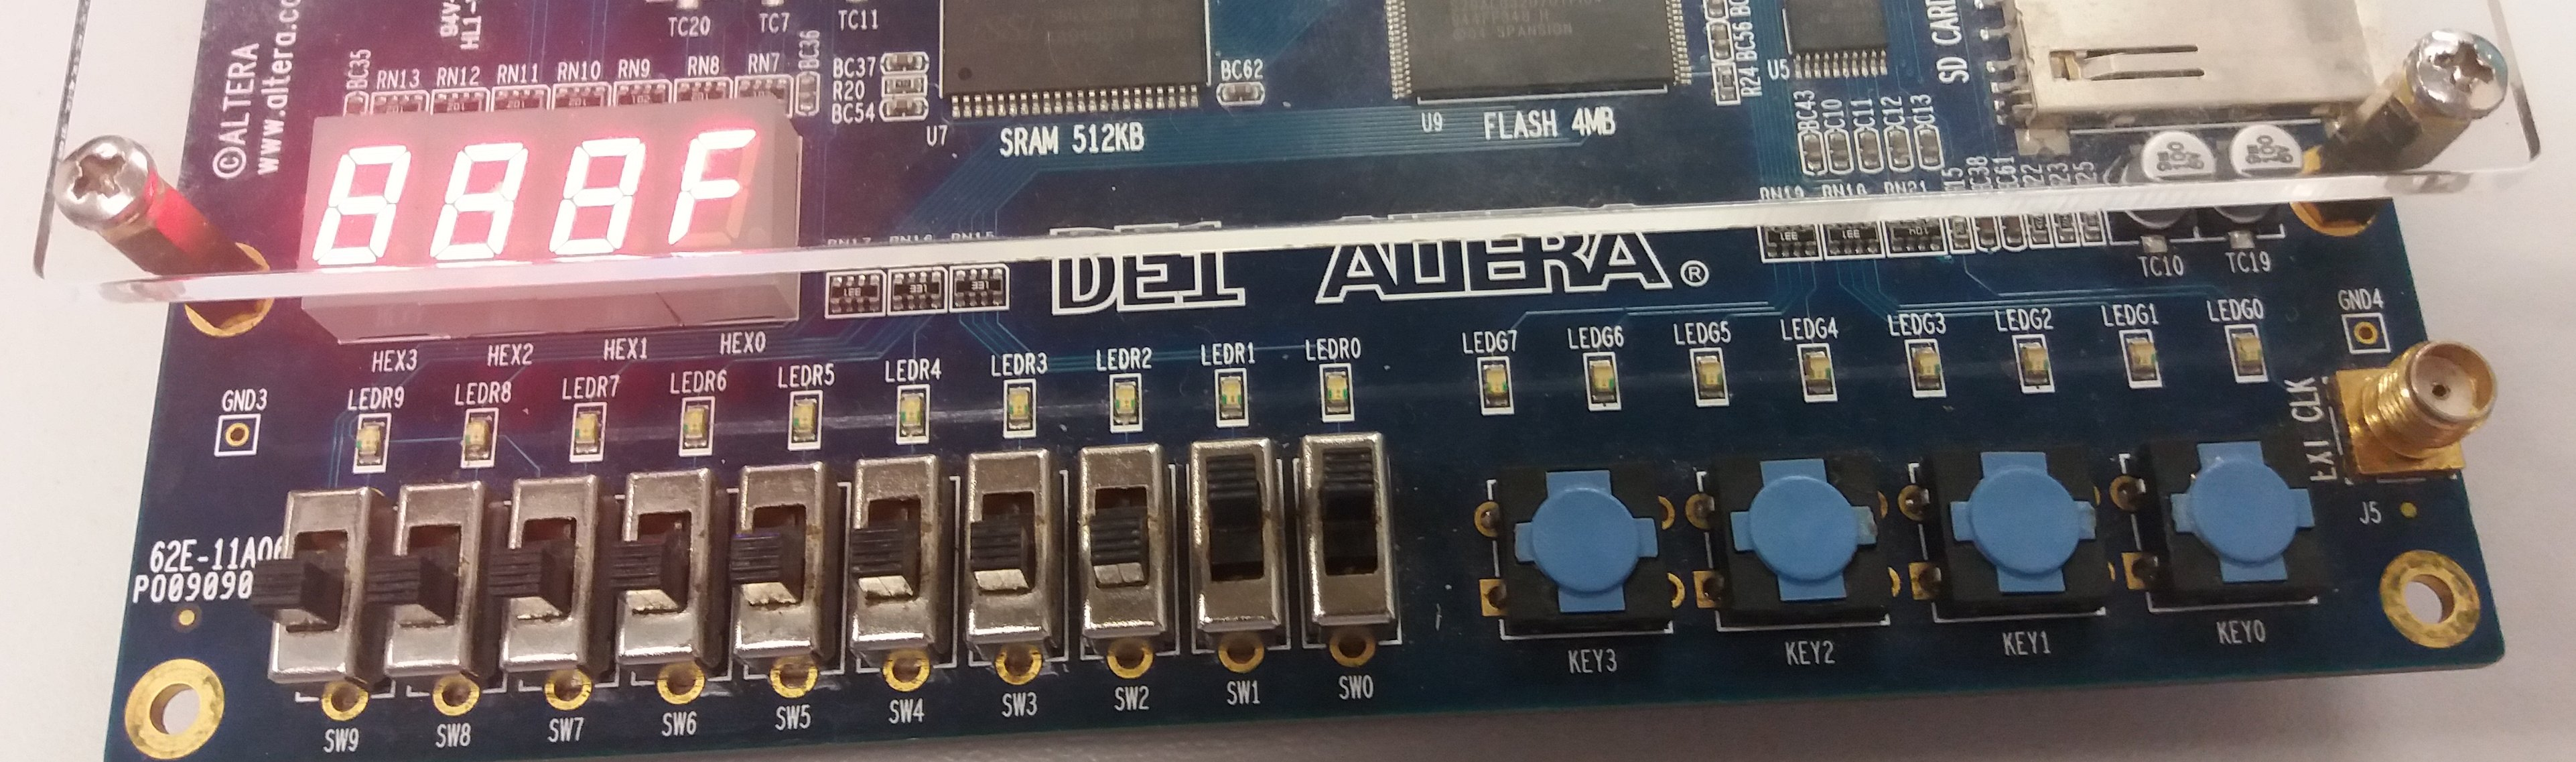
\includegraphics[width=\textwidth]{img/maquina/placa/Fechando-Fechado}
			\caption{Transição do estado Fechando para Fechado.}
		\end{subfigure}

		\caption{Teste do circuito rodando na placa.}\label{figura:deployMaquina}
	\end{figure}

%Apresentar os resultados da simulação em software e da utilização do Kit DE1 e/ou
%protoboard. Utilizar figuras, descrevê-las e discuti-las.
